\section{Decentralized information gathering}
\label{sec:infodecpomdp}
We next present our extension of the Dec-POMDP model for information-theoretic rewards.
Additionally, we motivate and discuss our assumption of periodic communication.

\subsection{Information-theoretic rewards for Dec-POMDPs}
Consider an information gathering task for a robot team.
It seems clear that an optimal policy should lead the robots to act such as to reach a state estimate with low uncertainty.
Reward functions that only depend on the state and action do not appear to be fully compatible with such objectives~\cite{Araya2010}.
For example, consider a robot team collecting information about a physical process which they are unable to affect through their actions, such as monitoring underwater ocean currents.
In this case, the underlying state is not meaningful for the robots' objective, nor are the possible actions by themselves.

In single-agent POMDPs, information gathering has been addressed, e.g., by augmenting the action space to include new actions that reward information-gathering~\cite{Spaan2010,Spaan2015}, or by applying information-theoretic rewards~\cite{Araya2010}.
The first approach results in a multiplication of the size of the agents' action spaces $\A_i$.
As the number of possible policies for an agent $i$ in a Dec-POMDP is $|\A_i|^{((|\A_i||\Z_i|)^h-1) / (|\A_i||\Z_i|-1))}$~\cite{Oliehoek2008}, this approach does not seem promising to translate to Dec-POMDPs.
We consider the second approach, which corresponds to setting a reward function that depends on the joint belief state instead of the true underlying state of the system.

In a Dec-POMDP, an individual agent usually cannot compute a joint belief state  based only on its local history.
However, during the centralized planning phase the possible joint histories $\theta_t$ are available, and each joint history corresponds to some joint belief state as indicated by Eq.~\eqref{eq:belief_update_history}.
Thus, information theoretic reward functions may be evaluated and applied in Dec-POMDPs while computing a joint policy.
Inspired by~\cite{Araya2010}, we call the resulting model a $\rho$Dec-POMDP.
\begin{definition}[$\rho$Dec-POMDP]
\label{def:rhodecpomdp}
A $\rho$Dec-POMDP is a tuple $\langle I$, $\St$, $\lbrace \A_i \rbrace_{i\in I}$, $\lbrace \Z_i \rbrace_{i\in I}$, $\T$, $\Ob$, $\rho$, $b_0 \rangle$, where $I$, $\St$, $\lbrace \A_i \rbrace_{i\in I}$, $\lbrace \Z_i \rbrace_{i\in I}$, $\T$, $\Ob$, and $b_0$ are as in the Dec-POMDP, and the reward function is $\rho:\B\times\A\to\R$.
\end{definition}
Choosing $\rho(b,a) = \sum\limits_{s\in\St}R(s,a)b(s)$, the definition above subsumes the standard Dec-POMDP (Definition~\ref{def:decpomdp}).
As in Eq.~\eqref{eq:decpolicy_value}, the value of a joint policy $\pi$ in a $\rho$Dec-POMDP is 
\begin{equation}
\label{eq:rhodecpolicy_value}
V(\pi) = \sum\limits_{t=0}^{h-1}\sum\limits_{\theta_t \in \Theta_t} P\left(\theta_t \,\middle|\, \pi, b_0 \right) \rho( \tau(\theta_t, b_0), \pi(\theta_t)),
\end{equation}
where $\tau(\theta_t, b_0)$ is the joint belief state computed by Eq.~\eqref{eq:belief_update_history}.

An appropriate reward function encourages the agents to reach joint histories corresponding to joint belief states with low uncertainty.
This is quantified via uncertainty functions.
\begin{definition}[Uncertainty function~\cite{DeGroot2004}]
Any non-negative, concave function $g:\B\to\R^+$ is applicable as an uncertainty function.
\end{definition}
An example of an uncertainty function is the Shannon entropy $H(b) = -\sum\limits_{s}b(s) \log_2 b(s)$~\cite{Cover2006}.
An uncertainty function has a small value for joint belief states near the degenerate case where all probability mass is concentrated on one state, and a greater value near the uniform distribution.

Throughout the remainder of the paper, we will consider $\rho$Dec-POMDP models with reward functions defined as
\begin{equation}
\label{eq:rhoreward}
\rho(b,a) = \sum\limits_{s\in\St}R(s,a)b(s) -\alpha g(b),
\end{equation}
where $R(s,a)$ models the rewards dependent on states and actions only, and $g$ is an uncertainty function encoding the information gathering objective\footnote{We apply a minus sign here to penalize for uncertainty in $b$.}.
The term $\alpha > 0$ sets the balance of state-dependent and information gathering rewards.

\subsection{Periodic communication}
Deploying a team of robots to collect information is useful if the collected information will eventually be combined to form a joint state estimate.
We assume the robots share data via periodic communication every $c$ time steps.
This leads to a scheme outlined in Figure~\ref{fig:decpolicy}.
Given an initial joint belief state, a joint policy is computed for a horizon $h$, and distributed to the agents for execution.
After $c$ time steps, the agents communicate to share their local histories, enabling estimation of a new joint belief state.
The new information may be applied to revise the joint policy.
The communication period $c$ need not be equal to the horizon $h$.

For $c=1$, information is immediately shared by all agents and the problem reduces to a multi-agent POMDP~\cite{Pynadath2002}.
The case $c>1$ is similar to the $k$-steps delayed communication case~\cite{Oliehoek2016}: at time $t$ all agents know $\theta_{t-k}$.
However, for periodic communication this information is obtained only during the communication intervals, instead of at every time step.

\begin{figure}[t]
\centering
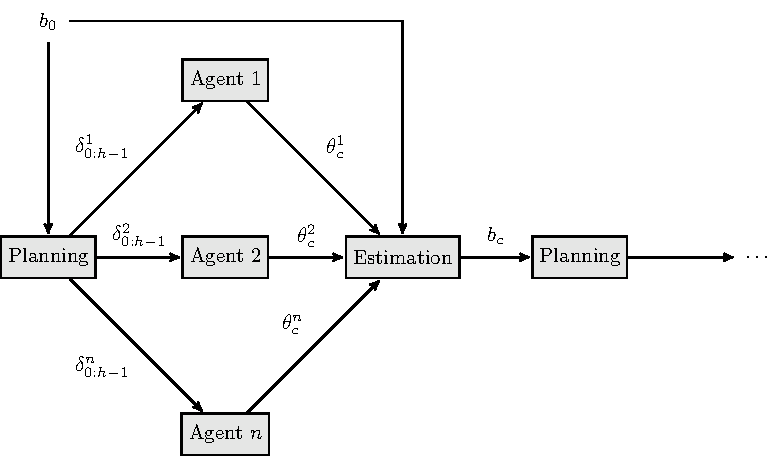
\includegraphics[width=0.8\columnwidth]{tikz/dec-policy/dec-policy.pdf}
\caption{Decentralized information gathering with communication period $c$. The agents act according to local decision rules $\delta_{0:h-1}^i$ for $c$ time steps ($c \leq h$), and then share their local histories $\theta_{c}^i$.
A joint belief state $b_{c}$ may then be estimated, and the information applied to plan subsequent actions.}
\label{fig:decpolicy}
\end{figure}

One might argue that it is sufficient to set a non-zero information reward $g$ only for the last time instant of the planning horizon.
While appropriate in some applications, a counterargument can be presented for applications such as the robot team monitoring ocean currents.
Here, we wish to estimate the state of the process accurately at all time steps to learn about the process dynamics.
In such cases, minimizing the ``average uncertainty'' via Eq.~\eqref{eq:rhoreward} is reasonable.